%==============================================================================
% Sjabloon poster bachproef
%==============================================================================
% Gebaseerd op document class `a0poster' door Gerlinde Kettl en Matthias Weiser
% Aangepast voor gebruik aan HOGENT door Jens Buysse en Bert Van Vreckem

\documentclass[a0,portrait]{hogent-poster}

% Info over de opleiding
\course{Bachelorproef}
\studyprogramme{toegepaste informatica}
\academicyear{2022-2023}
\institution{Hogeschool Gent, Valentin Vaerwyckweg 1, 9000 Gent}

% Info over de bachelorproef
\title{Scholieren met dyslexie van de derde graad middelbaar onderwijs ondersteunen bij het begrijpend lezen van wetenschappelijke artikelen via geautomatiseerde en gepersonaliseerde tekstvereenvoudiging.}
\subtitle{}
\author{Dylan Cluyse}
\email{dylan.cluyse@student.hogent.be}
\supervisor{Lena De Mol}
\cosupervisor{Johan Decorte (Hogeschool Gent); Jana Van Damme (Hogeschool Gent)}

% Indien ingevuld, wordt deze informatie toegevoegd aan het einde van de
% abstract. Zet in commentaar als je dit niet wilt.
\specialisation{AI en data engineering}
\keywords{Gepersonaliseerde tekstvereenvoudiging; dyslexie; natuurlijke taalverwerking}
\projectrepo{https://github.com/dylancluyse/bachelorproef-nlp-tekstvereenvoudiging}

\begin{document}

\maketitle

\begin{abstract}
Ingewikkelde woordenschat en zinsbouw hinderen scholieren met dyslexie in de derde graad van het middelbaar onderwijs bij het begrijpend lezen van wetenschappelijke artikelen. Gepersonaliseerde \textit{manual text simplification} (ATS) helpt deze scholieren bij hun leesbegrip. Daarnaast kan artificiële intelligentie (AI) dit proces automatiseren om de werkdruk bij leraren en scholieren te verminderen. Dit onderzoek achterhaalt met welke technologische en logopedische aspecten AI-ontwikkelaars rekening moeten houden bij de ontwikkeling van een AI-toepassing voor geautomatiseerde en gepersonaliseerde tekstvereenvoudiging. Hiervoor stelt het onderzoek de volgende onderzoeksvraag op: "Hoe kan een wetenschappelijk artikel automatisch worden vereenvoudigd, gericht op de unieke noden van scholieren met dyslexie in de derde graad middelbaar onderwijs?". Een requirementsanalyse achterhaalt de benodigde functionaliteiten om gepersonaliseerde en geautomatiseerde tekstvereenvoudiging mogelijk te maken. Vervolgens wijst de vergelijkende studie uit welk taalmodel ontwikkelaars kunnen inzetten om de taak van gepersonaliseerde en geautomatiseerde tekstvereenvoudiging mogelijk te maken. De requirementsanalyse wijst uit dat toepassingen om wetenschappelijke artikelen te vereenvoudigen, gemaakt zijn voor een centrale doelgroep en geen rekening houden met de unieke noden van een scholier met dyslexie in de derde graad middelbaar onderwijs. Toepassingen voor gepersonaliseerde \textit{automated text simplification} zijn mogelijk, maar ontwikkelaars moeten meer inzetten op de unieke noden van deze scholieren.
\end{abstract}

\begin{multicols}{2} % This is how many columns your poster will be broken into, a portrait poster is generally split into 2 columns

\section{Introductie}

Vindt u wetenschappelijke artikelen vermoeiend om te lezen? Storen het vakjargon, het compacte formaat u bij het begrijpend lezen van nieuw wetenschappelijk onderzoek? Dit is niet abnormaal, want het begrijpend lezen van wetenschappelijke artikelen vraagt een alsmaar grotere geletterdheid van de lezer. Alle doelgroepen krijgen het moeilijk te verduren, maar scholieren met dyslexie ervaren hier een nog grotere hindernis mee. Toch kunnen leerkrachten deze hindernis voor de studenten verwerpen, door teksten met \textit{manual text simplification} (MTS) te vereenvoudigen. Om de werkdruk in het onderwijs tegen te gaan, moet dit proces ook geautomatiseerd worden met \textit{automated text simplification} (ATS).


% Begrijpend lezen behoort tot de belangrijkste vaardigheden in het middelbaar onderwijs. Dagelijks moeten zij teksten kunnen doornemen en het tekstbegrip ervan onthouden. Scholieren met dyslexie kunnen moeilijkheden hebben bij het begrijpend lezen in het onderwijs. Daarnaast vraagt het begrijpend lezen van wetenschappelijke artikelen een alsmaar grotere geletterdheid van de lezer. Echter raken scholieren via deze bronnen in contact met wetenschappelijke onderzoek wat het aanleren van kritische vaardigheden met zich meebrengt. Leerkrachten kunnen deze wetenschappelijke artikelen vereenvoudigen op maat van deze scholieren. Dit proces noemt \textit{manual text simplification}. Zij kunnen MTS toepassen door ondersteunende woordenlijsten te maken, zinnen opnieuw te schrijven met een verminderde lexicale en syntactische complexiteit en de tekst te herschrijven als een opsomming of in tabelvorm. MTS past niets aan de oorspronkelijke semantiek aan. Hoewel dit een redmiddel kan zijn voor scholieren bij het begrijpend lezen van een wetenschappelijk artikel, toch is dit een proces dat tijd vergt van de personen die hierop MTS uitvoeren. Dit proces automatiseren met \textit{automatic text simplification} (ATS) is een haalbare taak met een capabel taalmodel, maar huidige toepassingen beschikken over onvoldoende functionaliteiten om gepersonaliseerde ATS aan te bieden. Dit onderzoek moet achterhalen hoe ontwikkelaars gepersonaliseerde ATS-functionaliteiten kunnen aanreiken in de vorm van een prototype.



\section{Onderzoeksmethoden}

Om een werkwijze te achterhalen voor het ontwikkelen van dergelijk toepassing, voert het onderzoek drie fasen uit weergegeven in figuur \ref{img:flowchart}.

\begin{center}
	\captionsetup{type=figure}
	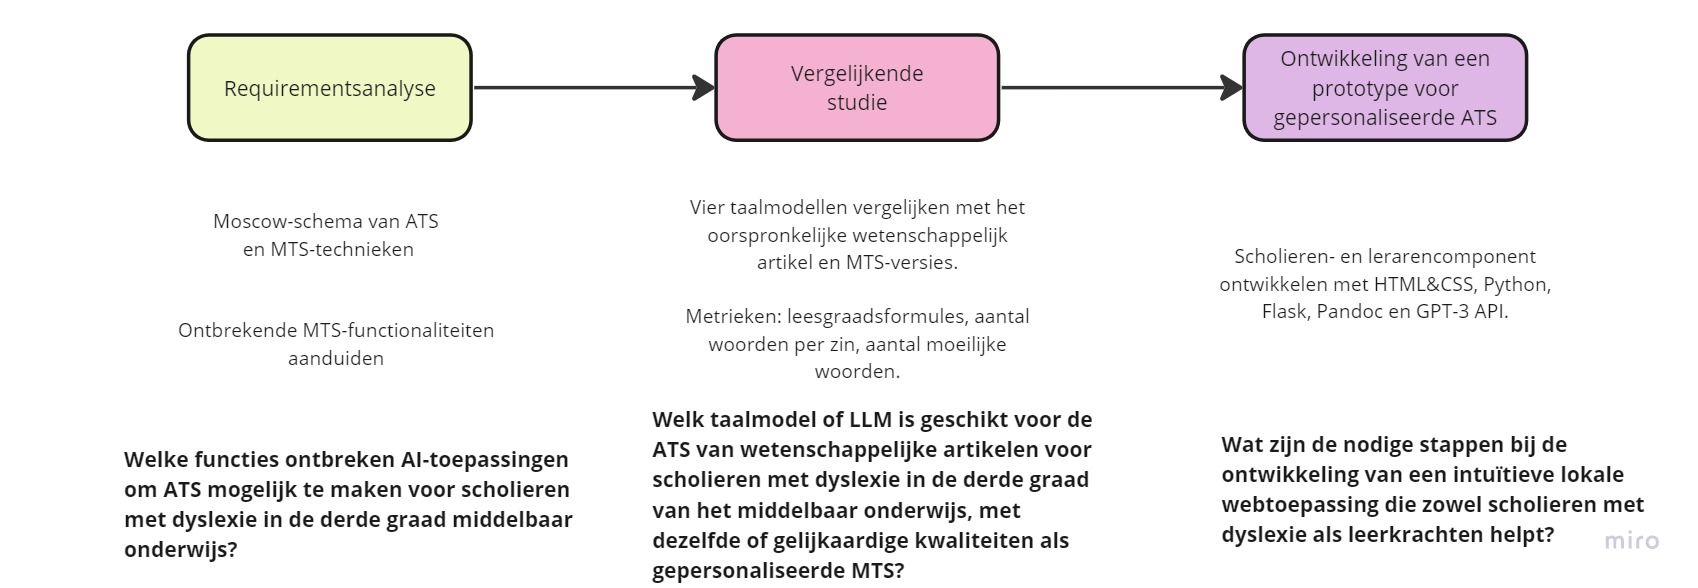
\includegraphics[width=1.0\linewidth]{figures/onderzoeksmethoden.jpg}
	\captionof{figure}{De gebruikte onderzoeksmethoden. In het vetgedrukt staan de onderzoeksvragen geschreven.}
	\label{img:flowchart}
\end{center}

% Allereerst achterhaalt het onderzoek met een requirementsanalyse de functionaliteiten voor gepersonaliseerde ATS bij huidige tools en toepassingen. Het resultaat van deze fase is een Moscow-schema met alle \textit{must-have} functionaliteiten tot alle \textit{wont-have} functionaliteiten. Dit beantwoordt de volgende onderzoeksvraag: Welke functies ontbreken AI-toepassingen om geautomatiseerde tekstvereenvoudiging mogelijk te maken voor scholieren met dyslexie in de derde graad middelbaar onderwijs? 

% Vervolgens moet het prototype beschikken over een geschikt taalmodel voor gepersonaliseerde ATS. Na de requirementsanalyse volgt een vergelijkende studie rond beschikbare taalmodellen om gepersonaliseerde ATS te kunnen realiseren. Het doel van deze onderzoeksmethode is om de beschikbare taalmodellen op HuggingFace en het GPT-3 taalmodel tegenover elkaar te plaatsen. Deze fase beantwoordt de volgende onderzoeksvraag: Welk taalmodel of LLM is geschikt voor de ATS van wetenschappelijke artikelen voor scholieren met dyslexie in de derde graad van het middelbaar onderwijs, met dezelfde of gelijkaardige kwaliteiten als gepersonaliseerde MTS?

% Tot slot volgt de ontwikkeling van het prototype. Het prototype maakt gebruik van vrij beschikbare technologieën en programmeertalen, zoals HTML/CSS en Python. Het prototype bestaat uit twee componenten. Enerzijds moet het prototype een ondersteunend middel bieden aan scholieren met dyslexie, door een wetenschappelijk artikel in een aanpasbaar formaat aan te bieden. Daarnaast kunnen scholieren aanpassingen aan de tekst maken, zoals weergegeven in figuur \ref{img:figure-1}. Dit beantwoordt de volgende onderzoeksvraag: Wat zijn de nodige stappen bij de ontwikkeling van een intuïtieve lokale webtoepassing die zowel scholieren met dyslexie als leerkrachten helpt?

\section{Uitwerking van het prototype}


% Allereerst achterhaalt het onderzoek met een requirementsanalyse de functionaliteiten voor gepersonaliseerde ATS bij huidige tools en toepassingen. Het resultaat van deze fase is een Moscow-schema met alle \textit{must-have} functionaliteiten tot alle \textit{wont-have} functionaliteiten. Deze requirementsanalyse onderzoekt de functionaliteiten bij huidige tools en toepassingen voor (gepersonaliseerde) ATS. Daarnaast achterhaalt de requirementsanalyse de ontbrekende MTS-technieken bij huidige toepassingen. De requirementsanalyse wijst de \textit{must-haves} waar het prototype voor gepersonaliseerde ATS over moet beschikken.

% Vervolgens moet het prototype beschikken over een geschikt taalmodel voor gepersonaliseerde ATS. Na de requirementsanalyse volgt een vergelijkende studie rond beschikbare taalmodellen om gepersonaliseerde ATS te kunnen realiseren. Het doel van deze onderzoeksmethode is om de beschikbare taalmodellen op HuggingFace en het GPT-3 taalmodel tegenover elkaar te plaatsen. Twee wetenschappelijke artikelen en twee MTS-vereenvoudigde teksten dienen als testmateriaal. Hier wordt gekeken welk taalmodel rekening houdt met gepersonaliseerde ATS, met gelijke kwaliteiten als MTS.

% Het prototype maakt gebruik van vrij beschikbare technologieën en programmeertalen, zoals HTML/CSS, Python en Het prototype bestaat uit twee componenten. Enerzijds kan het prototype een ondersteunend middel bieden aan scholieren met dyslexie, door een wetenschappelijk artikel in een aanpasbaar formaat aan te bieden. Daarnaast kunnen  

Scholieren kunnen de tekst aanpassen, zoals weergegeven in figuur \ref{img:figure-1}. Anderzijds kunnen leerkrachten een vereenvoudigde versie van een wetenschappelijk artikel laten maken met het prototype. Hier kan de leerkracht parameters meegeven, waaronder de opmaakopties en de vereenvoudigingen die de tekst moet aannemen.

\begin{center}
	\captionsetup{type=figure}
	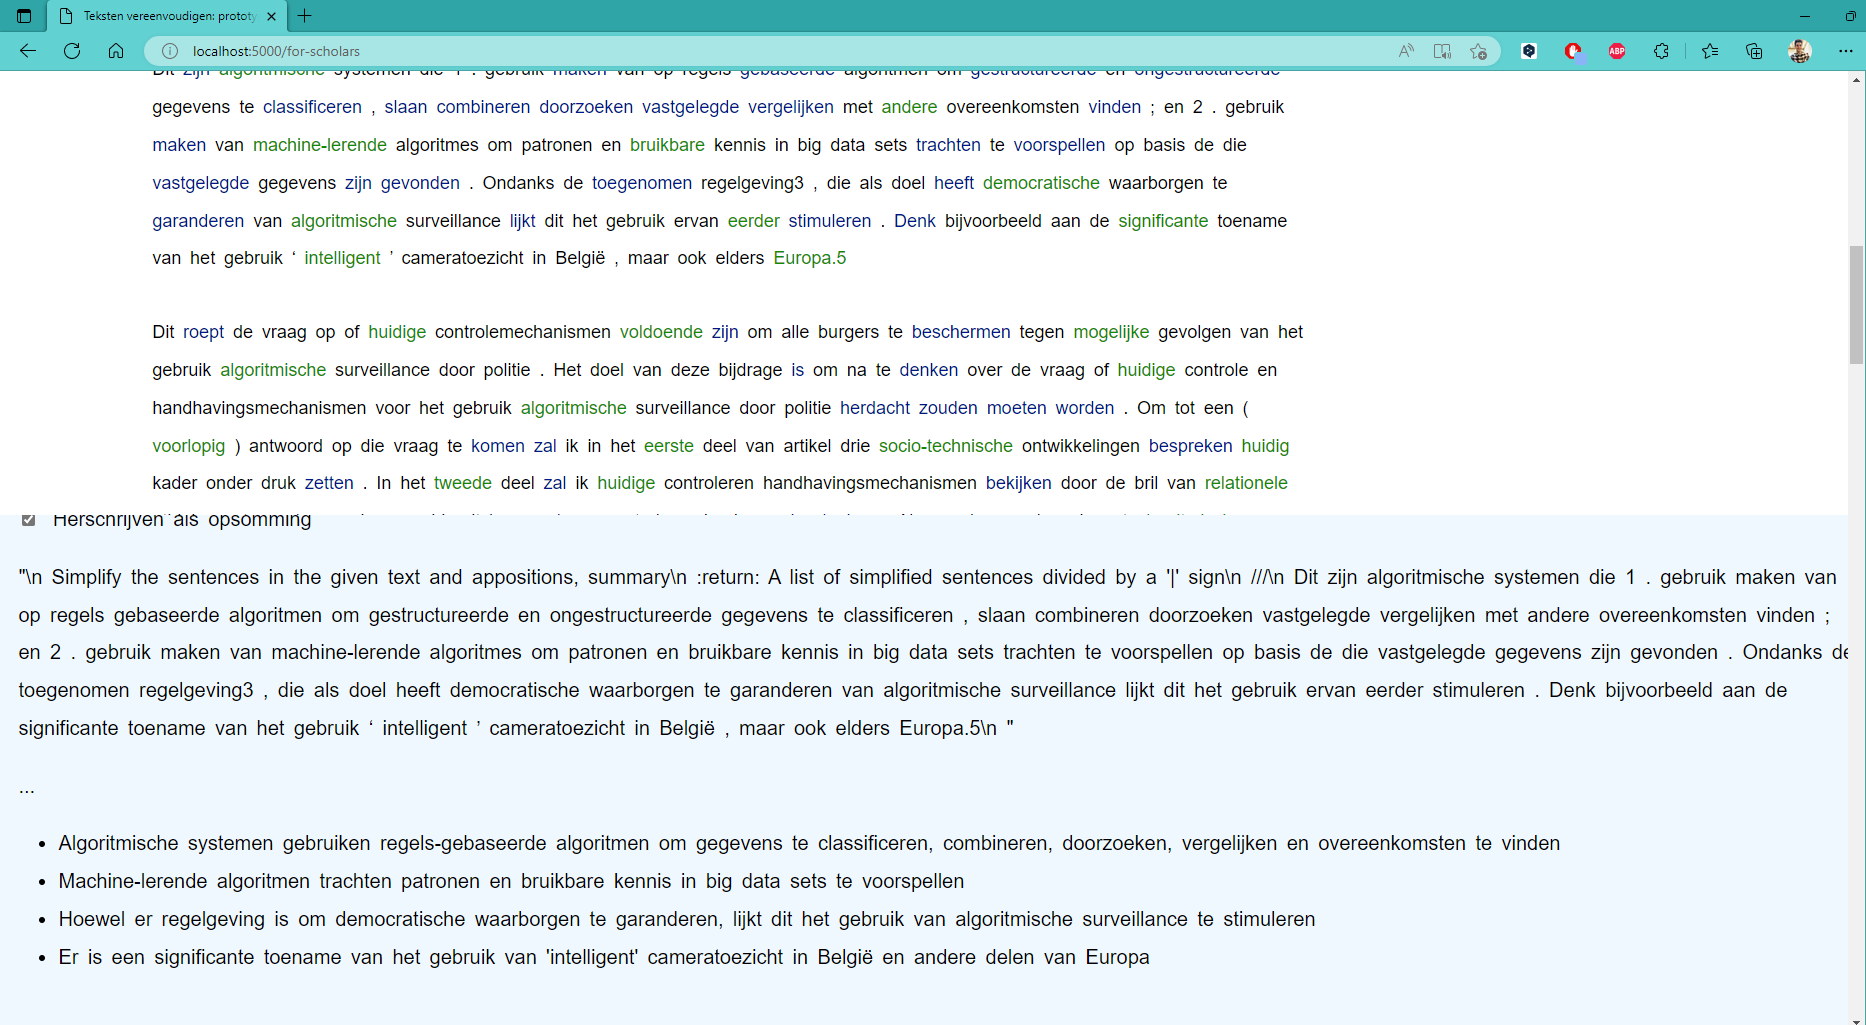
\includegraphics[width=1.0\linewidth]{figures/proto-opsomming-2.png}
	\captionof{figure}{Voorbeeldweergave van het scholierencomponent. De scholier selecteert een tekst en vraagt voor een opsomming (met eenvoudige woordenschat) van de gemarkeerde tekst.}
	\label{img:figure-1}
\end{center}

\section{Conclusies}

Uit de requirementsanalyse blijkt dat bestaande online tools en softwaretoepassingen voor ATS onvoldoende gepersonaliseerde functionaliteiten bieden. Ze missen opmaakopties voor scholieren met dyslexie. Recente technologieën bieden wel tekstvereenvoudigingsopties, maar vereisen informaticakennis die de meeste scholieren en leraren niet hebben. Een vergelijkende studie toont aan dat het GPT-3 taalmodel geschikt is voor LS en SS-technieken, terwijl andere taalmodellen minder coherente tekst genereren. Het prototype voor gepersonaliseerde ATS maakt gebruik van AI en NLP-technologieën zoals PDFMiner, de GPT-3 API en Pandoc. Hoewel het prototype nog niet aan alle functionaliteiten voldoet, kunnen ontwikkelaars met de gebruikte softwarepakketten een volledig afgewerkte toepassing ontwikkelen. 

\section{Toekomstig onderzoek}
% Verder onderzoek naar de toepassing van AI via een API, zoals het GPT-4 taalmodel, is noodzakelijk en kan baanbrekend zijn voor de onderwijssector. Dit onderzoek kan zich richten op doelgroepinschattingen via prompts en het potentieel van de combinatie van GPT-3 en \textit{full-text-search}-technologieën. Daarnaast is er behoefte aan onderzoek naar de verschillen tussen taalmodellen getraind op wetenschappelijke artikelen en taalmodellen getraind op algemene data. Tot slot kunnen logopedisten en studenten in deze richting het prototype gebruiken om verder onderzoek uit te voeren naar de effecten van gepersonaliseerde ATS bij scholieren met dyslexie in de derde graad van het middelbaar onderwijs. 

Figuur \ref{img:verder-onderzoek}

\begin{center}
	\captionsetup{type=figure}
	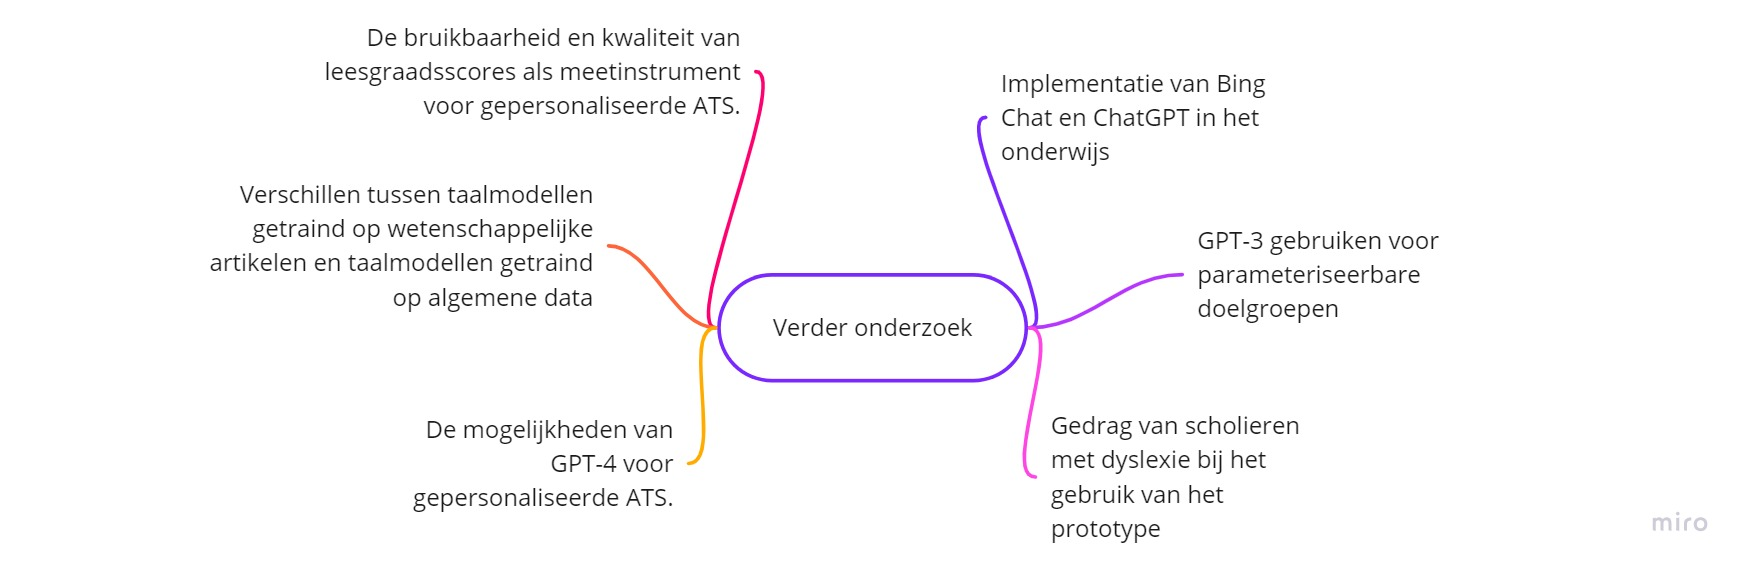
\includegraphics[width=1.0\linewidth]{figures/verder-onderzoek.jpg}
	\captionof{figure}{}
	\label{img:verder-onderzoek}
\end{center}


\end{multicols}
\end{document}